\documentclass[aspectratio=169,xcolor=table]{beamer}
\usetheme{Madrid}
\usepackage{amsmath,amssymb,booktabs}

\setbeamertemplate{navigation symbols}{}
\setbeamersize{text margin left=7mm,text margin right=7mm}

\title[SGD vs.\ R-SGD]{SGD versus Robust SGD\\under Gradient Uncertainty}
\date{}

\newcommand{\wideplot}[1]{%
    \includegraphics[width=\linewidth,height=0.79\textheight,keepaspectratio]{#1}}

\newcommand{\sweepplots}[1]{%
    \includegraphics[width=0.32\linewidth]{plots/#1/sgd_train_loss_vs_lr.pdf}\hfill
    \includegraphics[width=0.32\linewidth]{plots/#1/sgd_validation_loss_vs_lr.pdf}\hfill
    \includegraphics[width=0.32\linewidth]{plots/#1/learning_rate_schedule.pdf}}

\begin{document}

\begin{frame}
    \titlepage
\end{frame}

\section{Method and theory}

\begin{frame}{Gradient uncertainty}
    \begin{block}{Batch statistics}
        Observations \(v_{k,1},\ldots,v_{k,b}\) with sample covariance \(\widehat\Sigma_k\)
        \[
            g_k=\frac1b\sum_{i=1}^b v_{k,i},
            \qquad
            S_k=\frac{\operatorname{diag}(\widehat\Sigma_k)}{b}+\varepsilon I
        \]
    \end{block}
    \uncover<2->{
        \begin{block}{Ellipsoidal uncertainty set}
            \[
                \mathcal G_k=\{g_k+S_k^{1/2}u:\|u\|_2\le\rho\}
            \]
            Center \(g_k\), shape \(S_k\), radius \(\rho\)
        \end{block}
    }
\end{frame}

\begin{frame}{Robust update}
    \begin{block}{Worst-case linear loss change}
        \[
            \max_{h\in\mathcal G_k} h^\top d
            =g_k^\top d+\rho\|S_k^{1/2}d\|_2
        \]
    \end{block}
    \begin{block}{Unique step from a strongly convex subproblem}
        \[
            d_k=\arg\min_d
            \left\{g_k^\top d+\rho\|S_k^{1/2}d\|_2
                 +\frac{\|d\|_2^2}{2\alpha_k}\right\},
            \qquad \theta_{k+1}=\theta_k+d_k
        \]
    \end{block}
    \begin{center}
        \(\rho=0\): ordinary SGD, \(d_k=-\alpha_k g_k\)
    \end{center}
\end{frame}

\begin{frame}{Zero steps and isotropic shrinkage}
    \begin{alertblock}{Exact zero-step condition}
        \[
            d_k=0 \quad\Longleftrightarrow\quad
            \|S_k^{-1/2}g_k\|_2\le\rho
        \]
        Possible even away from a stationary point
    \end{alertblock}
    \begin{block}{Isotropic uncertainty: \(S_k=sI\)}
        \[
            d_k=-\alpha_k
            \left(1-\frac{\rho\sqrt{s}}{\|g_k\|_2}\right)_+g_k
            \qquad (g_k\ne 0)
        \]
        Nonzero step along \(-g_k\), length at most \(\alpha_k\|g_k\|_2\)
    \end{block}
\end{frame}

\begin{frame}{Anisotropy and conditional descent}
    \begin{block}{Optimality for \(d_k\ne 0\)}
        \[
            g_k+\rho\frac{S_kd_k}{r_k}+\frac{d_k}{\alpha_k}=0,
            \qquad r_k=\|S_k^{1/2}d_k\|_2
        \]
        For diagonal \(S_k\):
        \(\displaystyle
            (d_k)_j=-\frac{\alpha_k(g_k)_j}{1+\alpha_k\rho s_{k,j}/r_k}
        \)
    \end{block}
    \begin{block}{\(L\)-smooth loss and \(\nabla f(\theta_k)\in\mathcal G_k\)}
        \[
            f(\theta_k+d_k)\le f(\theta_k)-
            \left(\alpha_k^{-1}-L/2\right)\|d_k\|_2^2
        \]
        Strict decrease for \(d_k\ne 0\) and \(0<\alpha_k<2/L\)
    \end{block}
\end{frame}

\section{Implementation}

\begin{frame}{Inner solver selection: noisy quadratic, 100 repeats}
    \centering
    \small
    \setlength{\tabcolsep}{5pt}
    \begin{tabular}{lcrrrrr}
        \toprule
        Solver & Rel.\ tol. & Stop step
        & \shortstack{Time to stop\\(ms)}
        & \shortstack{Loss at stop\\(\(10^{-3}\))}
        & \shortstack{Loss at 500\\(\(10^{-4}\))}
        & \shortstack{Inner count\\(500 steps)} \\
        \midrule
        Brent & \(10^{-4}\) & 126.5 & \(20.3\pm16.5\) & \(4.52\pm7.96\) & \(2.27\pm2.79\) & 3410 \\
        \rowcolor{blue!10}
        \textbf{Brent} & \(\mathbf{10^{-2}}\) & 125.8 & \(15.1\pm7.1\) & \(4.52\pm7.96\) & \(2.27\pm2.79\) & 2774 \\
        Brent & \(10^{-1}\) & 126.9 & \(14.7\pm8.2\) & \(4.47\pm7.93\) & \(2.27\pm2.78\) & 2311 \\
        Brent & \(3\cdot10^{-1}\) & 161.7 & \(16.5\pm9.8\) & \(3.19\pm6.71\) & \(2.22\pm2.66\) & 1712 \\
        \midrule
        Proximal & \(10^{-4}\) & 126.5 & \(113.5\pm51.9\) & \(4.52\pm7.96\) & \(2.27\pm2.79\) & 23985 \\
        Proximal & \(10^{-2}\) & 125.6 & \(50.3\pm18.5\) & \(4.81\pm8.36\) & \(2.25\pm2.76\) & 10196 \\
        Proximal & \(10^{-1}\) & 114.4 & \(23.8\pm8.5\) & \(7.76\pm10.45\) & \(2.01\pm2.47\) & 3771 \\
        Proximal & \(3\cdot10^{-1}\) & 115.8 & \(14.7\pm5.3\) & \(24.72\pm18.00\) & \(4.41\pm4.81\) & 1486 \\
        \midrule
        Proximal (acc.) & \(10^{-4}\) & 126.5 & \(61.0\pm23.0\) & \(4.52\pm7.96\) & \(2.27\pm2.79\) & 11418 \\
        Proximal (acc.) & \(10^{-2}\) & 125.7 & \(20.0\pm8.6\) & \(4.57\pm8.02\) & \(2.28\pm2.80\) & 3025 \\
        Proximal (acc.) & \(10^{-1}\) & 112.2 & \(14.8\pm6.2\) & \(8.34\pm11.88\) & \(2.06\pm2.51\) & 1923 \\
        Proximal (acc.) & \(3\cdot10^{-1}\) & 114.1 & \(12.4\pm5.1\) & \(22.63\pm16.81\) & \(3.68\pm4.29\) & 1062 \\
        \bottomrule
    \end{tabular}
\end{frame}

\begin{frame}{Numerical checks}
    \begin{columns}[c,onlytextwidth]
        \begin{column}{0.59\textwidth}
            \centering
            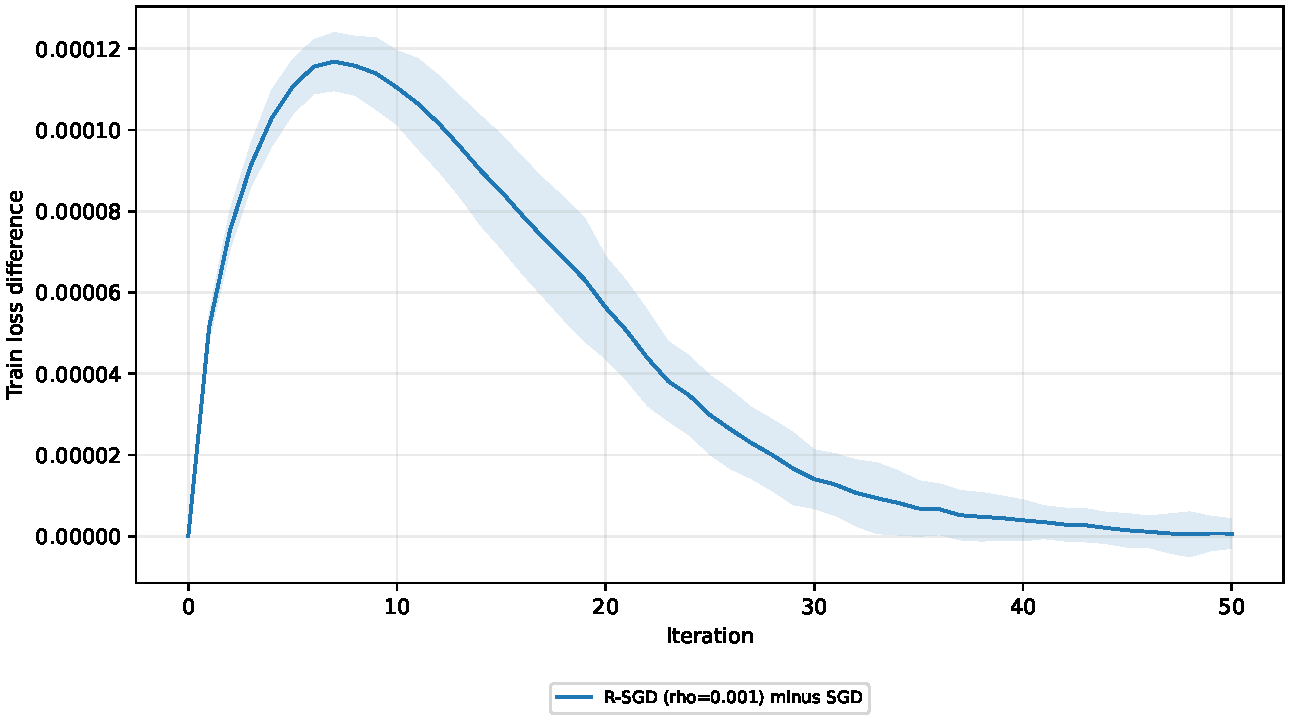
\includegraphics[width=\linewidth]{plots/zero_radius_check/train_loss_difference.pdf}
            \par\small Train loss difference (R-SGD minus SGD)\\
            \(\rho=10^{-3}\), 20 paired seeds, mean \(\pm\) SD
        \end{column}
        \begin{column}{0.38\textwidth}
            \small
            \begin{itemize}
                \item \(\rho=0\): exact match with SGD
                \item Isotropic step: max.\ error \(<1.5\cdot10^{-8}\)
                \item At \(\|S^{-1/2}g\|_2=1\):\\
                      nonzero at \(\rho=0.9\), zero at \(1\) and \(1.1\)
                \item Anisotropic step: max.\ relative residual \(<10^{-6}\)
            \end{itemize}
        \end{column}
    \end{columns}
\end{frame}

\begin{frame}{Effect of batch size}
    \framesubtitle{Noisy quadratic, 1,000 batches per size}
    \centering
    \[
        \operatorname{Cov}(g)=\Sigma/b,
        \qquad \operatorname{tr}(\Sigma)=4.25
    \]
    \renewcommand{\arraystretch}{1.2}
    \begin{tabular}{rrrr}
        \toprule
        \(b\) & \(\operatorname{tr}(S)\), mean \(\pm\) SD
        & \(b\) times mean trace & \(b\) times empirical trace \\
        \midrule
        8   & \(0.52794\pm0.26173\) & 4.2235 & 4.3441 \\
        32  & \(0.13308\pm0.03132\) & 4.2587 & 4.1182 \\
        128 & \(0.03332\pm0.00388\) & 4.2653 & 4.4307 \\
        512 & \(0.00832\pm0.00051\) & 4.2573 & 4.2204 \\
        \bottomrule
    \end{tabular}
    \vspace{1em}

    Ellipsoid axis lengths approximately proportional to \(b^{-1/2}\)
\end{frame}

\section{Experimental design}

\begin{frame}{Datasets and models}
    \framesubtitle{Binary cross-entropy, 512 / 256 / 512 training / validation / test examples}
    \begin{columns}[T,onlytextwidth]
        \begin{column}{0.48\textwidth}
            \begin{block}{Simulation 1: logistic regression}
                Gaussian classes, \(y\in\{0,1\}\)
                \[
                    a\sim\mathcal N((2y-1)(1,1)^\top,I_2)
                \]
                Logit \(w^\top a+c\)

                Zero initialization, 3 parameters
            \end{block}
        \end{column}
        \begin{column}{0.49\textwidth}
            \begin{block}{Simulation 2: two-layer network}
                Noisy semicircles, \(t\sim U[0,\pi]\)
                \[
                    (\cos t,\sin t),\quad (1-\cos t,\tfrac12-\sin t)
                \]
                Feature noise \(\mathcal N(0,0.1^2 I_2)\)

                Logit \(w_2^\top\tanh(W_1 a+b_1)+b_2\)

                8 hidden units, 33 parameters, Xavier initialization
            \end{block}
        \end{column}
    \end{columns}
\end{frame}

\begin{frame}{Paired tuning and evaluation}
    \small
    \begin{itemize}
        \item 500 updates, paired initializations, batch indices and noise draws
        \item Gradient observations \(v_{k,i}=u_i(\theta_k)+\sigma z_{k,i}\),
              \(z_{k,i}\sim\mathcal N(0,I)\)
        \item Tuning at \(b=64\): SGD schedule first, then R-SGD \((\alpha_0,\rho)\) on validation loss
        \item Frozen settings on separate seeds; batch sweep \(b\in\{16,64,256\}\) at \(\sigma=0\)
        \item Noise sweep at \(b=64\), plus \(b=16\) at the highest noise level
    \end{itemize}
    \begin{center}
        \begin{tabular}{lccc}
            \toprule
            Model & Repeats per setting & Tuning \(\sigma\) & Evaluation noise levels \\
            \midrule
            Logistic regression & 100 & 0.25 & \(0,\ 0.25,\ 0.5\) \\
            Two-layer network & 50 & 0.1 & \(0,\ 0.1,\ 0.2\) \\
            \bottomrule
        \end{tabular}
    \end{center}
    \begin{block}{Stopping statistics alongside the fixed budget}
        First hit: five consecutive steps with \(\|d_k\|_2\le 10^{-3}(1+\|\theta_k\|_2)\)
    \end{block}
\end{frame}

\section{Logistic regression}

\begin{frame}{Logistic regression: SGD learning rates}
    \framesubtitle{500 updates, mean \(\pm\) sample SD across 100 runs}
    \centering
    \sweepplots{logistic}

    \vspace{0.8em}
    \(\alpha=0.1\) selected for SGD, constant schedule for both methods
\end{frame}

\begin{frame}{Logistic regression: R-SGD training grid}
    \framesubtitle{Mean training loss at update 500}
    \centering
    \renewcommand{\arraystretch}{1.25}
    \setlength{\tabcolsep}{4pt}
    \begin{tabular}{rrrrrrrrr}
\hline
$\alpha_0$ & $\rho=0$ & $\rho=0.05$ & $\rho=0.125$ & $\rho=0.25$ & $\rho=0.5$ & $\rho=1$ & $\rho=2$ & $\rho=4$ \\
\hline
$0.03$ & $0.19103$ & $0.19155$ & $0.19236$ & $0.19377$ & $0.19684$ & $0.20400$ & $0.22216$ & $0.26951$ \\
$0.1$ & $0.16920$ & $0.16937$ & $0.16964$ & $0.17015$ & $0.17144$ & $0.17544$ & $0.19069$ & $0.23857$ \\
$0.3$ & $0.16598$ & $\mathbf{0.16598}$ & $0.16598$ & $0.16600$ & $0.16608$ & $0.16677$ & $0.17480$ & $0.21981$ \\
$0.7$ & $0.16646$ & $0.16644$ & $0.16640$ & $0.16634$ & $0.16621$ & $0.16600$ & $0.16827$ & $0.20814$ \\
$1.5$ & $0.16749$ & $0.16745$ & $0.16738$ & $0.16727$ & $0.16706$ & $0.16669$ & $0.16624$ & $0.19895$ \\
$3$ & $0.16943$ & $0.16933$ & $0.16919$ & $0.16896$ & $0.16855$ & $0.16789$ & $0.16673$ & $0.19135$ \\
\hline
\end{tabular}

\end{frame}

\begin{frame}{Logistic regression: R-SGD validation grid}
    \framesubtitle{Mean validation loss at update 500}
    \centering
    \renewcommand{\arraystretch}{1.18}
    \setlength{\tabcolsep}{4pt}
    \begin{tabular}{rrrrrrrrr}
\hline
$\alpha_0$ & $\rho=0$ & $\rho=0.05$ & $\rho=0.125$ & $\rho=0.25$ & $\rho=0.5$ & $\rho=1$ & $\rho=2$ & $\rho=4$ \\
\hline
$0.03$ & $0.21736$ & $0.21774$ & $0.21833$ & $0.21937$ & $0.22167$ & $0.22723$ & $0.24211$ & $0.28375$ \\
$0.1$ & $\mathbf{0.20615}$ & $0.20616$ & $0.20618$ & $0.20624$ & $0.20653$ & $0.20808$ & $0.21751$ & $0.25638$ \\
$0.3$ & $0.20902$ & $0.20896$ & $0.20886$ & $0.20868$ & $0.20824$ & $0.20712$ & $0.20805$ & $0.24048$ \\
$0.7$ & $0.21067$ & $0.21066$ & $0.21066$ & $0.21064$ & $0.21057$ & $0.21004$ & $0.20679$ & $0.23102$ \\
$1.5$ & $0.21172$ & $0.21171$ & $0.21169$ & $0.21166$ & $0.21164$ & $0.21172$ & $0.20917$ & $0.22394$ \\
$3$ & $0.21411$ & $0.21402$ & $0.21389$ & $0.21368$ & $0.21335$ & $0.21308$ & $0.21255$ & $0.21842$ \\
\hline
\end{tabular}

    \vspace{0.6em}

    \begin{block}{Selected R-SGD setting: \(\rho=2\), \(\alpha=0.7\)}
        Validation loss \(0.20679\) vs.\ \(0.20615\) at the grid minimum
    \end{block}
\end{frame}

\begin{frame}{Logistic regression: radius sensitivity}
    \framesubtitle{Fixed \(\alpha=0.1\), \(b=64\), \(\sigma=0.25\)}
    \centering
    \small
    \renewcommand{\arraystretch}{1.12}
    \begin{tabular}{rrrrrr}
        \toprule
        \(\rho\) & Train loss & Zero steps (\%) & Relative step length & Hits & Time (ms) \\
        \midrule
        0     & \(0.1691\pm0.0005\) & \(0.00\pm0.00\) & \(1.000\pm0.000\) & 1/100    & \(51.4\pm29.5\) \\
        0.05  & \(0.1693\pm0.0005\) & \(0.00\pm0.00\) & \(0.968\pm0.001\) & 1/100    & \(96.6\pm21.4\) \\
        0.25  & \(0.1701\pm0.0005\) & \(0.23\pm0.25\) & \(0.845\pm0.004\) & 17/100   & \(80.0\pm13.8\) \\
        0.5   & \(0.1713\pm0.0006\) & \(1.59\pm0.57\) & \(0.704\pm0.006\) & 63/100   & \(74.6\pm22.2\) \\
        1     & \(0.1753\pm0.0006\) & \(9.36\pm1.13\) & \(0.480\pm0.007\) & 100/100  & \(45.8\pm14.4\) \\
        2     & \(0.1905\pm0.0009\) & \(30.69\pm1.70\) & \(0.243\pm0.004\) & 100/100 & \(29.0\pm8.3\) \\
        4     & \(0.2383\pm0.0015\) & \(55.16\pm1.55\) & \(0.098\pm0.002\) & 100/100 & \(18.6\pm6.9\) \\
        \bottomrule
    \end{tabular}

    \medskip
    Time to first hit or update 500, averaged over all runs
\end{frame}

\begin{frame}{Logistic regression: results at update 500}
    \framesubtitle{Mean \(\pm\) sample SD across 100 runs}
    \centering
    \small
    \setlength{\tabcolsep}{3pt}
    \resizebox{\linewidth}{!}{\begin{tabular}{rrlrrrrrr}
\hline
$b$ & $\sigma$ & Method & Train loss & Test loss & Acc. (\%) & Time (ms) & Zero (\%) & Grad. eval. \\
\hline
16 & 0 & SGD & $0.1692 \pm 0.0005$ & $0.1905 \pm 0.0010$ & $92.80 \pm 0.20$ & $38.7 \pm 5.7$ & $0.00 \pm 0.00$ & $8000 \pm 0$ \\
16 & 0 & R-SGD & $0.1667 \pm 0.0006$ & $0.1944 \pm 0.0015$ & $92.98 \pm 0.19$ & $56.5 \pm 2.5$ & $46.71 \pm 1.98$ & $8000 \pm 0$ \\
64 & 0 & SGD & $0.1691 \pm 0.0002$ & $0.1906 \pm 0.0006$ & $92.82 \pm 0.14$ & $39.7 \pm 4.9$ & $0.00 \pm 0.00$ & $32000 \pm 0$ \\
64 & 0 & R-SGD & $0.1664 \pm 0.0003$ & $0.1940 \pm 0.0009$ & $92.77 \pm 0.19$ & $56.3 \pm 5.8$ & $49.44 \pm 1.86$ & $32000 \pm 0$ \\
256 & 0 & SGD & $0.1690 \pm 0.0001$ & $0.1904 \pm 0.0003$ & $92.82 \pm 0.09$ & $48.3 \pm 7.0$ & $0.00 \pm 0.00$ & $128000 \pm 0$ \\
256 & 0 & R-SGD & $0.1665 \pm 0.0002$ & $0.1932 \pm 0.0005$ & $92.69 \pm 0.14$ & $66.9 \pm 8.2$ & $45.07 \pm 1.69$ & $128000 \pm 0$ \\
64 & 0.25 & SGD & $0.1691 \pm 0.0005$ & $0.1907 \pm 0.0009$ & $92.79 \pm 0.20$ & $39.1 \pm 3.1$ & $0.00 \pm 0.00$ & $32000 \pm 0$ \\
64 & 0.25 & R-SGD & $0.1681 \pm 0.0007$ & $0.1916 \pm 0.0014$ & $92.77 \pm 0.26$ & $54.0 \pm 9.6$ & $62.22 \pm 1.76$ & $32000 \pm 0$ \\
64 & 0.5 & SGD & $0.1692 \pm 0.0010$ & $0.1910 \pm 0.0016$ & $92.78 \pm 0.27$ & $42.1 \pm 7.8$ & $0.00 \pm 0.00$ & $32000 \pm 0$ \\
64 & 0.5 & R-SGD & $0.1693 \pm 0.0016$ & $0.1914 \pm 0.0023$ & $92.78 \pm 0.28$ & $50.3 \pm 2.9$ & $66.52 \pm 1.84$ & $32000 \pm 0$ \\
16 & 0.5 & SGD & $0.1699 \pm 0.0023$ & $0.1913 \pm 0.0030$ & $92.78 \pm 0.34$ & $37.4 \pm 2.8$ & $0.00 \pm 0.00$ & $8000 \pm 0$ \\
16 & 0.5 & R-SGD & $0.1706 \pm 0.0036$ & $0.1934 \pm 0.0051$ & $92.75 \pm 0.34$ & $47.9 \pm 3.1$ & $66.01 \pm 1.89$ & $8000 \pm 0$ \\
\hline
\end{tabular}
}
\end{frame}

\begin{frame}{Logistic regression: stopping statistics}
    \framesubtitle{First-hit statistics among hits, update 500 for zero-hit rows}
    \centering
    \small
    \begin{tabular}{rrlrrrrr}
\hline
$b$ & $\sigma$ & Method & Hits & Update & Time (ms) & Acc. (\%) & Failed \\
\hline
16 & 0 & SGD & 1/100 & $479.0$ & $36.0$ & $92.77$ & 0 \\
16 & 0 & R-SGD & 100/100 & $119.7 \pm 50.8$ & $14.9 \pm 5.9$ & $93.00 \pm 0.21$ & 0 \\
64 & 0 & SGD & 80/100 & $414.8 \pm 51.6$ & $33.3 \pm 5.8$ & $92.89 \pm 0.16$ & 0 \\
64 & 0 & R-SGD & 100/100 & $115.0 \pm 38.6$ & $14.9 \pm 4.7$ & $93.09 \pm 0.14$ & 0 \\
256 & 0 & SGD & 100/100 & $268.3 \pm 18.9$ & $26.3 \pm 5.9$ & $93.02 \pm 0.09$ & 0 \\
256 & 0 & R-SGD & 100/100 & $125.0 \pm 23.9$ & $19.8 \pm 5.8$ & $93.01 \pm 0.09$ & 0 \\
64 & 0.25 & SGD & 1/100 & $453.0$ & $34.1$ & $92.97$ & 0 \\
64 & 0.25 & R-SGD & 100/100 & $70.7 \pm 23.6$ & $9.2 \pm 3.0$ & $93.06 \pm 0.18$ & 0 \\
64 & 0.5 & SGD & 0/100 & $500.0 \pm 0.0$ & $42.1 \pm 7.8$ & $92.78 \pm 0.27$ & 0 \\
64 & 0.5 & R-SGD & 100/100 & $48.1 \pm 18.7$ & $6.0 \pm 2.1$ & $93.04 \pm 0.29$ & 0 \\
16 & 0.5 & SGD & 0/100 & $500.0 \pm 0.0$ & $37.4 \pm 2.8$ & $92.78 \pm 0.34$ & 0 \\
16 & 0.5 & R-SGD & 100/100 & $43.1 \pm 21.4$ & $5.0 \pm 2.3$ & $92.89 \pm 0.49$ & 0 \\
\hline
\end{tabular}

\end{frame}

\begin{frame}{Logistic regression: added gradient noise}
    \framesubtitle{\(b=64\), mean \(\pm\) SD from update 200}
    \centering
    \wideplot{plots/logistic/noise_losses.pdf}
\end{frame}

\begin{frame}{Logistic regression: batch size}
    \framesubtitle{Training loss by updates and by example gradients, \(\sigma=0\)}
    \centering
    \wideplot{plots/logistic/batch_losses.pdf}
\end{frame}

\begin{frame}{Logistic regression: decision boundaries}
    \framesubtitle{Test set, evaluation seed 1042, update 500}
    \centering
    \wideplot{plots/logistic/decision_boundaries.pdf}
\end{frame}

\section{Two-layer network}

\begin{frame}{Two-layer network: SGD learning rates}
    \framesubtitle{500 updates, mean \(\pm\) sample SD across 50 runs}
    \centering
    \sweepplots{network}

    \vspace{0.8em}
    \(\alpha_0=6\) selected for SGD, schedule \(\alpha_k=\alpha_0/\sqrt{1+k/50}\) for both methods
\end{frame}

\begin{frame}{Two-layer network: R-SGD training grid}
    \framesubtitle{Mean training loss at update 500}
    \centering
    \renewcommand{\arraystretch}{1.12}
    \setlength{\tabcolsep}{4pt}
    \begin{tabular}{rrrrrrrrr}
\hline
$\alpha_0$ & $\rho=0$ & $\rho=0.5$ & $\rho=1$ & $\rho=2$ & $\rho=3$ & $\rho=4$ & $\rho=6$ & $\rho=8$ \\
\hline
$0.03$ & $0.32005$ & $0.32298$ & $0.32625$ & $0.33369$ & $0.34222$ & $0.35176$ & $0.37374$ & $0.39955$ \\
$0.1$ & $0.24531$ & $0.24701$ & $0.24921$ & $0.25489$ & $0.26189$ & $0.26991$ & $0.28896$ & $0.31242$ \\
$0.3$ & $0.23021$ & $0.23086$ & $0.23157$ & $0.23312$ & $0.23555$ & $0.24044$ & $0.25875$ & $0.28024$ \\
$0.7$ & $0.17793$ & $0.18710$ & $0.19740$ & $0.21477$ & $0.22647$ & $0.23197$ & $0.24553$ & $0.26694$ \\
$1.5$ & $0.07787$ & $0.09157$ & $0.10497$ & $0.13379$ & $0.17626$ & $0.21512$ & $0.23709$ & $0.25810$ \\
$3$ & $0.02655$ & $0.04308$ & $0.05744$ & $0.07696$ & $0.10125$ & $0.15107$ & $0.23249$ & $0.25114$ \\
$6$ & $\mathbf{0.00601}$ & $0.00673$ & $0.00746$ & $0.01567$ & $0.05575$ & $0.10264$ & $0.21815$ & $0.24441$ \\
$12$ & $0.01716$ & $0.01932$ & $0.01374$ & $0.00958$ & $0.01432$ & $0.02955$ & $0.11584$ & $0.24121$ \\
$24$ & $0.09765$ & $0.09664$ & $0.07070$ & $0.06365$ & $0.05646$ & $0.08390$ & $0.16918$ & $0.38641$ \\
\hline
\end{tabular}

\end{frame}

\begin{frame}{Two-layer network: R-SGD validation grid}
    \framesubtitle{Mean validation loss at update 500}
    \centering
    \renewcommand{\arraystretch}{1.08}
    \setlength{\tabcolsep}{4pt}
    \begin{tabular}{rrrrrrrrr}
\hline
$\alpha_0$ & $\rho=0$ & $\rho=0.5$ & $\rho=1$ & $\rho=2$ & $\rho=3$ & $\rho=4$ & $\rho=6$ & $\rho=8$ \\
\hline
$0.03$ & $0.31991$ & $0.32266$ & $0.32572$ & $0.33274$ & $0.34084$ & $0.34999$ & $0.37136$ & $0.39680$ \\
$0.1$ & $0.25199$ & $0.25342$ & $0.25531$ & $0.26034$ & $0.26661$ & $0.27376$ & $0.29081$ & $0.31241$ \\
$0.3$ & $0.24251$ & $0.24303$ & $0.24353$ & $0.24433$ & $0.24551$ & $0.24889$ & $0.26444$ & $0.28317$ \\
$0.7$ & $0.19220$ & $0.20125$ & $0.21139$ & $0.22843$ & $0.23961$ & $0.24394$ & $0.25354$ & $0.27185$ \\
$1.5$ & $0.09078$ & $0.10509$ & $0.11901$ & $0.14833$ & $0.19080$ & $0.22915$ & $0.24732$ & $0.26466$ \\
$3$ & $0.03543$ & $0.05306$ & $0.06834$ & $0.08984$ & $0.11533$ & $0.16584$ & $0.24496$ & $0.25913$ \\
$6$ & $\mathbf{0.00998}$ & $0.01118$ & $0.01244$ & $0.02310$ & $0.06725$ & $0.11607$ & $0.23221$ & $0.25383$ \\
$12$ & $0.03331$ & $0.03520$ & $0.02398$ & $0.02077$ & $0.02810$ & $0.04446$ & $0.14245$ & $0.25660$ \\
$24$ & $0.17291$ & $0.16375$ & $0.12888$ & $0.11672$ & $0.09979$ & $0.13327$ & $0.22581$ & $0.45727$ \\
\hline
\end{tabular}

    \vspace{0.4em}

    \begin{block}{Selected R-SGD setting: \(\rho=1\), \(\alpha_0=6\)}
        Validation loss \(0.01244\) vs.\ \(0.00998\) at the grid minimum
    \end{block}
\end{frame}

\begin{frame}{Two-layer network: radius sensitivity}
    \framesubtitle{Fixed \(\alpha_0=6\), \(b=64\), \(\sigma=0.1\)}
    \centering
    \small
    \renewcommand{\arraystretch}{1.10}
    \begin{tabular}{rrrrrr}
        \toprule
        \(\rho\) & Train loss & Zero steps (\%) & Relative step length & Hits & Time (ms) \\
        \midrule
        0   & \(0.0065\pm0.0012\) & \(0.00\pm0.00\) & \(1.000\pm0.000\) & 0/50  & \(74.8\pm11.8\) \\
        0.5 & \(0.0071\pm0.0014\) & \(0.00\pm0.00\) & \(0.907\pm0.003\) & 0/50  & \(114.4\pm19.7\) \\
        1   & \(0.0083\pm0.0021\) & \(0.00\pm0.00\) & \(0.815\pm0.006\) & 0/50  & \(117.6\pm19.7\) \\
        2   & \(0.0222\pm0.0443\) & \(0.00\pm0.00\) & \(0.634\pm0.012\) & 0/50  & \(122.0\pm14.4\) \\
        3   & \(0.0615\pm0.0727\) & \(0.02\pm0.07\) & \(0.449\pm0.020\) & 0/50  & \(123.7\pm21.1\) \\
        4   & \(0.1176\pm0.0777\) & \(3.53\pm1.66\) & \(0.270\pm0.019\) & 0/50  & \(111.7\pm16.8\) \\
        6   & \(0.2224\pm0.0206\) & \(58.27\pm2.73\) & \(0.055\pm0.006\) & 50/50 & \(10.0\pm7.1\) \\
        8   & \(0.2460\pm0.0060\) & \(88.36\pm1.60\) & \(0.012\pm0.002\) & 50/50 & \(3.9\pm2.3\) \\
        \bottomrule
    \end{tabular}

    \medskip
    Time to first hit or update 500, averaged over all runs
\end{frame}

\begin{frame}{Two-layer network: results at update 500}
    \framesubtitle{Mean \(\pm\) sample SD across 50 runs}
    \centering
    \small
    \setlength{\tabcolsep}{3pt}
    \resizebox{\linewidth}{!}{\begin{tabular}{rrlrrrrrr}
\hline
$b$ & $\sigma$ & Method & Train loss & Test loss & Acc. (\%) & Time (ms) & Zero (\%) & Grad. eval. \\
\hline
16 & 0 & SGD & $0.0068 \pm 0.0023$ & $0.0054 \pm 0.0022$ & $99.95 \pm 0.11$ & $73.1 \pm 4.4$ & $0.00 \pm 0.00$ & $8000 \pm 0$ \\
16 & 0 & R-SGD & $0.0482 \pm 0.0870$ & $0.0458 \pm 0.0857$ & $98.09 \pm 4.29$ & $103.6 \pm 3.7$ & $0.00 \pm 0.03$ & $8000 \pm 0$ \\
64 & 0 & SGD & $0.0062 \pm 0.0011$ & $0.0053 \pm 0.0014$ & $99.99 \pm 0.04$ & $82.5 \pm 4.3$ & $0.00 \pm 0.00$ & $32000 \pm 0$ \\
64 & 0 & R-SGD & $0.0301 \pm 0.0630$ & $0.0285 \pm 0.0611$ & $98.97 \pm 3.05$ & $113.1 \pm 3.3$ & $0.02 \pm 0.09$ & $32000 \pm 0$ \\
256 & 0 & SGD & $0.0066 \pm 0.0037$ & $0.0060 \pm 0.0036$ & $99.99 \pm 0.05$ & $125.3 \pm 15.5$ & $0.00 \pm 0.00$ & $128000 \pm 0$ \\
256 & 0 & R-SGD & $0.0163 \pm 0.0353$ & $0.0154 \pm 0.0344$ & $99.68 \pm 1.62$ & $157.8 \pm 9.0$ & $0.01 \pm 0.04$ & $128000 \pm 0$ \\
64 & 0.1 & SGD & $0.0065 \pm 0.0012$ & $0.0058 \pm 0.0015$ & $99.95 \pm 0.09$ & $85.6 \pm 5.8$ & $0.00 \pm 0.00$ & $32000 \pm 0$ \\
64 & 0.1 & R-SGD & $0.0083 \pm 0.0021$ & $0.0074 \pm 0.0022$ & $99.98 \pm 0.06$ & $118.1 \pm 4.4$ & $0.00 \pm 0.00$ & $32000 \pm 0$ \\
64 & 0.2 & SGD & $0.0078 \pm 0.0022$ & $0.0074 \pm 0.0022$ & $99.86 \pm 0.14$ & $84.3 \pm 4.6$ & $0.00 \pm 0.00$ & $32000 \pm 0$ \\
64 & 0.2 & R-SGD & $0.0087 \pm 0.0023$ & $0.0079 \pm 0.0020$ & $99.91 \pm 0.13$ & $122.7 \pm 9.7$ & $0.00 \pm 0.00$ & $32000 \pm 0$ \\
16 & 0.2 & SGD & $0.0161 \pm 0.0108$ & $0.0154 \pm 0.0084$ & $99.59 \pm 0.26$ & $77.1 \pm 7.8$ & $0.00 \pm 0.00$ & $8000 \pm 0$ \\
16 & 0.2 & R-SGD & $0.0168 \pm 0.0092$ & $0.0146 \pm 0.0085$ & $99.64 \pm 0.33$ & $111.0 \pm 6.5$ & $0.00 \pm 0.00$ & $8000 \pm 0$ \\
\hline
\end{tabular}
}
\end{frame}

\begin{frame}{Two-layer network: stopping statistics}
    \framesubtitle{First-hit statistics among hits, update 500 for zero-hit rows}
    \centering
    \small
    \begin{tabular}{rrlrrrrr}
\hline
$b$ & $\sigma$ & Method & Hits & Update & Time (ms) & Acc. (\%) & Failed \\
\hline
16 & 0 & SGD & 48/50 & $302.1 \pm 82.7$ & $44.9 \pm 12.3$ & $99.93 \pm 0.13$ & 0 \\
16 & 0 & R-SGD & 29/50 & $388.6 \pm 77.7$ & $80.6 \pm 17.0$ & $99.89 \pm 0.16$ & 0 \\
64 & 0 & SGD & 41/50 & $393.7 \pm 63.9$ & $64.9 \pm 11.6$ & $99.99 \pm 0.06$ & 0 \\
64 & 0 & R-SGD & 26/50 & $422.8 \pm 55.4$ & $96.5 \pm 13.2$ & $99.99 \pm 0.04$ & 0 \\
256 & 0 & SGD & 35/50 & $405.6 \pm 63.0$ & $102.6 \pm 23.5$ & $100.00 \pm 0.00$ & 0 \\
256 & 0 & R-SGD & 41/50 & $368.1 \pm 73.6$ & $117.0 \pm 22.8$ & $100.00 \pm 0.03$ & 0 \\
64 & 0.1 & SGD & 0/50 & $500.0 \pm 0.0$ & $85.6 \pm 5.8$ & $99.95 \pm 0.09$ & 0 \\
64 & 0.1 & R-SGD & 0/50 & $500.0 \pm 0.0$ & $118.1 \pm 4.4$ & $99.98 \pm 0.06$ & 0 \\
64 & 0.2 & SGD & 0/50 & $500.0 \pm 0.0$ & $84.3 \pm 4.6$ & $99.86 \pm 0.14$ & 0 \\
64 & 0.2 & R-SGD & 0/50 & $500.0 \pm 0.0$ & $122.7 \pm 9.7$ & $99.91 \pm 0.13$ & 0 \\
16 & 0.2 & SGD & 0/50 & $500.0 \pm 0.0$ & $77.1 \pm 7.8$ & $99.59 \pm 0.26$ & 0 \\
16 & 0.2 & R-SGD & 0/50 & $500.0 \pm 0.0$ & $111.0 \pm 6.5$ & $99.64 \pm 0.33$ & 0 \\
\hline
\end{tabular}

\end{frame}

\begin{frame}{Two-layer network: added gradient noise}
    \framesubtitle{\(b=64\), mean \(\pm\) SD from update 200}
    \centering
    \wideplot{plots/network/noise_losses.pdf}
\end{frame}

\begin{frame}{Two-layer network: batch size}
    \framesubtitle{Training loss by updates and by example gradients, \(\sigma=0\)}
    \centering
    \wideplot{plots/network/batch_losses.pdf}
\end{frame}

\begin{frame}{Two-layer network: decision boundaries}
    \framesubtitle{Test set, evaluation seed 1042, update 500}
    \centering
    \wideplot{plots/network/decision_boundaries.pdf}
\end{frame}

\section{Conclusions}

\begin{frame}{Conclusions}
    \begin{itemize}
        \setlength{\itemsep}{0.65em}
        \item \textbf{SGD at 500 updates:} lower mean test loss in 11/12 settings,
              faster in 12/12
        \item \textbf{With added noise:} smaller test-loss gap at \(b=64\) in both models
        \item<2-> \textbf{Large radii:} more zero steps, earlier rule hits, higher training loss
        \item<2-> \textbf{Prediction:} different rankings by training loss and test accuracy
        \item<2-> \textbf{Next check:} robust step length with SGD direction,
                   same gradient budget
    \end{itemize}
\end{frame}

\end{document}
